\section{Tensor Algebra Methods to Reduce Computational Complexity in Quantum Chemistry}
	A tensor is a multidimensional array; an N-th order tensor can considered as a outer product of N vector spaces. A first order tensor is an array, a second order tensor is a matrix and tensor of order three or higher is referred to as a higher-order tensor.\cite{Kolda2008}. Tensors are naturally applied single reference quantum mechanics: operators such as \textbf{F} can be expressed in terms of two electron coordinate products and form second order tensors while other operators and amplitudes such as the coulomb repulsion operator, $\hat{J}$, and the cluster operator amplitudes, $t^{ij\dots}_{ab\dots}$, can be expressed as higher-order tensor whose order depends on the number of indices's.  This extension therefore means as number of electrons increase, there is an exponential increase in the amount of storage and computational processing required to solve a given problem.  This problem is referred to as the "curse of dimensionality" %find a curse of dimensionality paper!%
	 To overcome this curse requires one to discover the underlying structure in data to reduce storage requirements and to redesign algorithms to scale with the structure of the data.\\
	The goal of a decomposition is to reduce the complexity of a tensor utilizing the underlying form of data in a tensor.  The result of a tensor decomposition provide information on the relative importance and weighting of individual vector spaces.  Direct methods to compute second order, matrix decompositions, such as the Singular Value, LU, and Jordan decomposition, have been around for quite some time.  Though, interests to decompose higher order tensors didn't develop until 1927 with Hitchcock's idea of a tensor to be a polyadic sum of products\cite{Hitchcock 1927, Hitchcock 1928} and later Cattells's idea of a multi-way model in 1944\cite{Cattell 1944, Cattell 1952}. These ideas would later be used to develop canonical product(CP) (CANDECOMP/PARAFAC canonical decomposition / parallel factor decomposition) \cite{Carroll 1970, Harshman 1970} and Tucker decompositions\cite{Tucker 1966}.  In order to apply ab initio quantum mechanics to larger systems and circumvent the "curse of dimensionality" it is necessary to take advantage of matrix and higher order tensor decomposition approximations and to redesign canonical algorithms using tensors in decomposed form. To follow are theoretical chemist's current tools to approximate and reduce the complexity of large systems while preserving accuracy.

	\subsection{Cholesky Decomposition}
		The Cholesky decomposition (CD) was first applied to quantum chemistry and specifically the two electron integral (TEI) tensor in 1977 by Beeble and Linderberg\cite{Beeble 1977} when the authors realized that, coupled with the positive definite nature of the integrals values, one could to reorder the higher-order tensor into a lower order object and perform a matrix decomposition.  What makes the CD special is that it can remove small and zero eigenvalues without calculating the entire matrix, providing computational savings.  CD has been in conjunction with two electron geminal implementation, derivative integrals and more recently has been applied to large scale TEI decomposition\cite{Aquilante 2011}.\\
		CD works by using a partial lower-upper(LU) decomposition of any two electron tensor recast into a symmetric positive definite matrix 
			\begin{equation}
				\begin{aligned}
					\label{eqn:CD}
					M_{\mu\nu, \gamma\sigma} = \int \int \rho_{\mu\nu}(r_1)\hat{M}(r_1,r_2) \rho_{\gamma\sigma} dr_1 dr_2 \equiv (\rho_{\mu\nu}|\rho_{\gamma\sigma})
				\end{aligned}
			\end{equation}
		where $\rho_{\mu\nu} = \phi_\mu\phi_\nu$ is an orbital density product and $\hat{M}(r_1,r_2)$ is some two electron operator. With the goal of expressing
			\begin{equation}
				M = BB^T
			\end{equation}
		This expression can be approximated to some decomposition threshold, $\gamma$, therefore elements of M can be expressed as
			\begin{equation}
				\begin{aligned}
					M_{\mu\nu, \gamma\sigma} \approx \sum_{p=1}^{P} B_{\mu\nu}^P B_{\gamma\sigma}^P &= \sum_{p=1}^{P} (\rho_{\mu\nu}|B_p)(B_p|\rho_{\gamma\sigma})\\
					&= \sum_{pq} (\rho_{\mu\nu}|b_p)(\hat{M}(r_1,r_2)^{-1})_{pq}(b_q|\rho_{\gamma\sigma})
				\end{aligned}
			\end{equation}
		where P is the rank of the decomposition which depends on $\gamma$.  A comprehensive CD algorithm is presented by Epifanovsky et al\cite{Epifanovsky 2013} which can be used to find optimal Cholesky basis, $b_p$, for a given $\hat{M}(r_1,r_2)$
	\subsection{Density Fitting}
		Density fitting (DF) is an specific application of CD where a canonical optimized Cholesky basis is used to decompose the TEI tensor into two third order tensors.  The roots of DF have been grounded in Coulomb\cite{Ten-no 1995, Vahtras 1993} and Exchange\cite{Weigend 2002} fitting in Hartree-Fock and has been applied to MP2\cite{Feyereisen 1993}, CCSD(T)\cite{Rendell 1994} and even explicitly correlated methods\cite{Manby 2003}.  The derivation of DF to proceed will be based on equations presented by Werner et al.\cite{Werner 2003}. The goal of DF is to decompose the TEI tensor
			\begin{equation}
				\begin{aligned}
			\olap{\mu\gamma}{\nu\sigma} = (\mu\nu|\gamma\sigma) &= \int\frac{\phi_\mu(r_1) \phi_\nu(r_1) \phi_\gamma(r_2)\phi_\sigma(r_2)}{r_{12}} dr_1 dr_2\\
			&= \int \frac{\rho_{\mu\nu}(r_1)\rho_{\gamma\sigma}(r_2)}{r_{12}}dr_1 dr_2
				\end{aligned}
			\end{equation}
		one electron densities, $\rho_{\mu\nu}(r) = \phi_\mu(r) \phi_\nu(r)$, can then be approximated as 
			\begin{equation}
				\bar{\rho_{\mu\nu}}(r) = \sum_A^{N_{fit}} d^{\mu\nu}_A \chi_A(r)
			\end{equation}
		where $\chi_A(r)$ are fitting basis functions and expansion coefficients, $d^{\mu\nu}_A$, can be found by minimizing the functional 
			\begin{equation}
				\Delta_{\mu\nu} = \int dr_1 \int dr_2 \frac{(\rho_{\mu\nu}(r_1)-\bar{\rho}_{\mu\nu}(r_1)) - (\rho_{\mu\nu}(r_2) - \bar{\rho}_{\mu\nu}(r_2))}{r_{12}}
			\end{equation}
		which provides 
			\begin{equation}
				d^{\mu\nu}_B = \sum_B (\mu\nu|A)[J^{-1}]_{AB}
			\end{equation}
		where 
			\begin{equation}
				(\mu\nu|A) = \int dr_1 \int dr_2 \frac{\phi_\mu(r_1)\phi_\nu(r_1)\chi_A(r_2)}{r_{12}}
			\end{equation}
		The term J is chosen to be some metric, here it is defined as the coulomb metric\cite{Dunlap 1977, Dunlap 1979}
			\begin{equation}
				J_{AB} = \int dr_1 \int dr_2 \frac{\chi_A(r_1) \chi_B(r_2)}{r_{12}}
			\end{equation}
		other metrics have been proposed\cite{Baerends 1973} and though they are less accurate, these metrics are computed more quickly than the Coulomb metric.\\
		This allows one to express the TEI as 
			\begin{equation}
				(\mu\nu|\gamma\sigma) = \sum_B d^{\mu\nu}_B (B|\gamma\sigma) = \sum_{AB} (\mu\nu|A)[J^{-1}]_{AB}(B|\gamma\sigma)
			\end{equation}
		transforming $J^{-1} = J^{-1/2}J^{-1/2}$ allows one to store the TEI as two third order tensors, reducing storage requirements from $\mathcal{O}(N^4)$ to $\mathcal{O}(N^2\cdot N_{fit}) \approx \mathcal{O}(N^3)$; $N_{fit}$ typically scales linearly with basis set.  Additionally one finds reduction in computational effort in calculations such as the Coulomb term, $\hat{J}$, in HF and transforming integrals from the AOs to MOs in MP2 calculations.\\
		To further reduce the complexity and storage of DF one can choose to use only a subset of the given auxiliary basis.  Original construction of subsets was based on distance based domains. Unfortunately this led to discontinuities on the potential energy surface.  Recently it has been shown that a better method is to only include fitting functions for a density,$\rho_{\mu\nu}$, where $\mu$ and $\nu$ are centered on the same point. This method is referred to as Concentric Atomic Density Fitting.  This idea combined with a localization method and inclusion of exact semi-diagonal terms to reduce complexity in calculation and storage of the coulomb, $\hat{J}$, and exchange term, $\hat{K}$ in HF by Hollman et al\cite{Hollman}
	\subsection{Direct Tensor Decomposition methods}
		In the case of matrices, applications of decomposition methods are straightforward and imply the transformation to some canonical form based on the rank of the matrix.  The extensions of decompositions to higher order tensors is not simple.  The rank of a tensor is defined as the smallest number of rank one tensors that generate the tensor as its sum, where a rank one tensor is defined as
			\begin{equation}
				\mathit{X} = a^{(1)} \otimes a^{(2)} \otimes \dots \otimes a^{(N)}
			\end{equation}
		where
			\begin{equation}
				\begin{aligned}
					\mathit{X} &\in \mathbb{R}^{I_1I_2\dots I_N} \\
					a^{(1)} \in \mathbb{R}^{I_1}, \quad a^{(2)} &\in \mathbb{R}^{I_2}, \quad \dots, \quad a^{(N)} \in \mathbb{R}^{(N)}
				\end{aligned}
			\end{equation}
		and a rank R tensor, $\mathit{U}$ can be defined in the canonical format (CP)
			\begin{equation}
				\mathit{U} = \sum_{r=1}^R \lambda_r a^{(1)}_r \otimes a^{(2)}_r \otimes \dots \otimes a^{(N)}_r \quad \lambda_r \in \mathbb{R}
			\end{equation}
		where $a^{(l)}_i$ are normalized vectors and one can then define the factor matrices as $A^{(l)} = [a_1,\dots a_r]\quad l\in\{1,2,\dots,N\}$.  Though it is not necessary to require each factor matrix have the same rank therefore one can also define the Tucker format (also refered to as the higher order singular value decomposition, HOSVD)
			\begin{equation}
				\mathit{U} = \sum_{\alpha_1}^{r_1} \dots \sum_{\alpha_N}^{r_N} \beta_{\alpha_1\dots\alpha_N}a_{\alpha_1}^{(1)}\otimes \dots \otimes a_{\alpha_N}^{(N)}
			\end{equation}
		where $\{ a_{\alpha_i}^{(l)}\}$ are a set of orthonormal vectors and $\beta \in \mathbb{R}^{r_1,r_2,\dots r_n}$ is the Tucker core tensor
	  Unlike matrix decompositions, there are no concise method to calculate the rank of a tensor, solving the rank is an NP hard problem\cite{Hastad1990}.  Though there are many schemes which can solve for the approximate rank of a tensor, $\mathit{T}$, by iteratively minimizing a series of non-linear equations\cite{Kolda 2008}
	  	\begin{equation}
	  		\begin{aligned}
	  			\|\mathit{T} - \mathit{U}\| < \epsilon
	  		\end{aligned}
	  	\end{equation}
	  where $\mathcal{U}$ is defined using canonical or Tucker format. Figure's 2 and 3 depict diagrammatically the CP and Tucker format\\
	  \begin{figure}
		\centering
			\begin{minipage}{.5\textwidth}
			  \centering
			  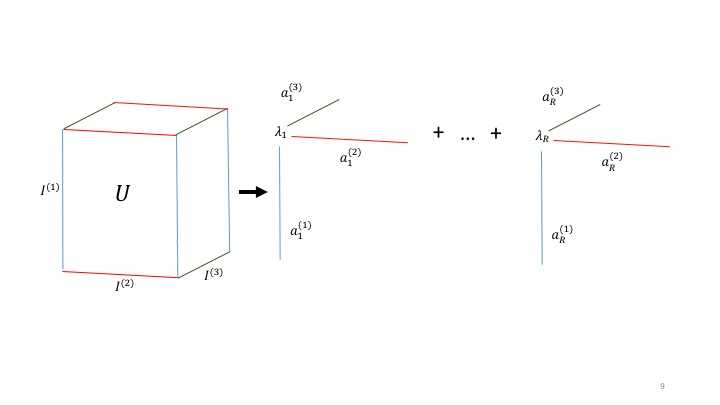
\includegraphics[width=1\linewidth]{./pics/CP_picture.jpg}
			  \captionof{figure}{Pictorial representation of CP format}
			  \label{fig:Figure 2}
			\end{minipage}%
			\begin{minipage}{.5\textwidth}
			  \centering
			  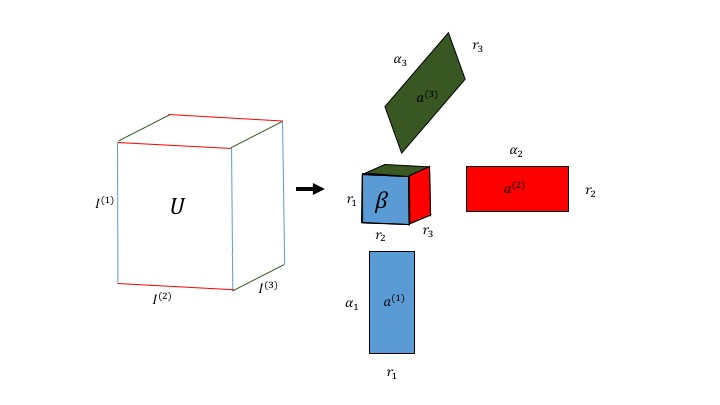
\includegraphics[width=1 \linewidth]{./pics/Tucker_picture.jpg}
			  \captionof{figure}{Pictorial representation of Tucker format}
			  \label{fig:Figure 3}
			\end{minipage}
		\end{figure}

	  Historically, the Tucker decomposition can be linked to complete active-space self-consistent field (CASSCF) method\cite{Roos 1980}, where excitation amplitude decomposition yields optimized orbitals for each tensor, and the CP decomposition can be linked to full CI\cite{Bell 2010} (FCI) where methods such as perfect pairing approach can be considered rank one tensor approximations to the FCI tensor. The idea of using CP decomposition for FCI has recently resurfaced\cite{Uemura 2012, Bohm 2016}. Today, there is an effort to make use of element sparsity in higher dimension to decompose tensors in canonical ab initio methods. In work presented by Benedikt et al\cite{Benedikt 2011, Benedikt 2013, Benedikt 2014}, post-HF operator and amplitude tensors are decomposed to compute MP2 and CCD using CP format for example
	  	\begin{equation}
	  		(\mu\nu|\rho\sigma) = \sum_r^R \chi^{(\mu)}_r \otimes \chi^{(\nu)}_r \otimes \chi^{(\rho)}_r \otimes \chi^{(\sigma)}_r
	  	\end{equation}
	  Using this form the authors developed equations which preserve decomposed form and rank.  These methods allow for reduced complexity in storage with out significant trade-off in accuracy and reduce the computational effort to perform any tensor contraction to $K \cdot d \cdot R1 \cdot R2$where K is the number of orbitals, d is the dimension of the tensors, and R1 and R2 are the ranks of each tensor. Unfortunately, finding the CP decomposition for tensors such as the TEI is non-trivial and costly and each tensor contraction increases storage requirements. Therefore, implementation of CP decomposed post-HF methods are not yet desirable.

	  In work presented by Bell et al\cite{Bell 2010} truncated HOSVD is employed to decompose the MP2 method $T_2$ amplitude expression, 
	  	\begin{equation}
	  		T_2(i,a,j,b) = \frac{(ia|jb)}{\epsilon_i + \epsilon_j - \epsilon_a - \epsilon_b}
	  	\end{equation}
	  This author showed that HOSVD could reduce storage of $T_2$ amplitudes for MP2 energy recovery from 85 to 99\%.  Additionally, they showed that orbital active spaces obtained through the HOSVD coincide with physical intuition based on how the tensor is unfolded, in the first step of the HOSVD algorithm.  Though the HOSVD does have some downsides, first HOSVD alone does not provide an optimal basis in terms of energy recovery it must therefore be coupled with other tensor decompositions and the algorithm to compute the HOSVD scales asymptotically as $\mathcal{O}(N^5)$\cite{Bell 2010}.

	\subsection{Tensor Hypercontraction}
		Tensor Hypercontraction (THC) was introduced in 2012 by Hohenstein, Parrish and Martinez\cite{Schutski}.  THC can be though of as a tensors decompositions applied to a DF decomposition, though in practice a CD or DF is not required. The THC for the TEI for example can be formulated a number of ways.  As an example a TCH on a general four index tensor (FIT) will be derived.  THC's goal is to recompose the FIT as a connected product of matrices 
			\begin{equation}
				V_{pqrs} \approx W_{p,\alpha} W_{q,\alpha} X_{\alpha\beta} W_{\beta, r} W_{\beta,s}
			\end{equation}
		First the step is to rewritten the FIT aa two index tensor
			\begin{equation}
				V_{pqrs} = V_{pq,rs}
			\end{equation}
		Then using an SVD one can express the two index tensor as
			\begin{equation}
				V_{pq,rs} = U_{pq,r_{SVD}}S_{\lambda,\lambda} V^T_{\lambda, rs}
			\end{equation}
		where $\lambda$ is the rank of the decomposition.  Here one may choose to use a truncated SVD or a CD or DF.  The singular values are then rerepresented as $S = S^{1/2} S^{1/2}$ and multiplied into the left and right singular vectors.
			\begin{equation}
				V_{pq,rs} = \tilde{U}_{pq, \lambda} \tilde{V}^T_{\lambda,rs}
			\end{equation}
		If one uses the CD or DF, a matrix roots of the overlap, $J^{1/2}$ of $J_{\lambda,\lambda}$ must be found to using an eigenvalue decomposition or SVD. Next, a CP decomposition is then performed on the three index tensors $\tilde{U}$ and $\tilde{V}$
			\begin{equation}
				\begin{aligned}
					\tilde{U}_{pq, \lambda} = W_{p,\alpha} W_{q, \alpha} W_{\alpha, \lambda}\\
					\tilde{V}^T_{\lambda,rs} = W_{\lambda, \beta} W_{\beta, r} W_{\beta, s}
				\end{aligned}
			\end{equation}
		where $\alpha$ and $\beta$ are the rank of the CP decomposition.  So far only applications where $\alpha = \beta$ have been studied. Finally the terms $W_{\alpha, \lambda} \text{ and } W_{\lambda, \beta}$ are contracted and one finds
			\begin{equation}
				V_{pqrs} = U_{p, \alpha} W_{q, \alpha} W_{\alpha, \beta} W_{\beta, r} W_{\beta, s}
			\end{equation}
		THC has been used in the field to represent the electron interaction potentials in CC2 methods and to decompose the TEI and calculate CCSD and FCI energies. In work presented by Hummel et al \cite{Hummel} THC was used to reduce the computational scaling of distinguishable CCD or linearlized CCSD from $\mathcal{O}(N^6)$ to $\mathcal{O}(N^5)$ and in work presented by Schutski et al\cite{Schutski} computational scaling of CCSD was reduced to $\mathcal{O}(N^4)$.  Schutski also presents a direct THC method which allows TEI decomposition to scale as $\mathcal{O}(N^5)$ using the SVD or $\mathcal{O}(N^4)$ using a DF scheme while preserving accuracy of \~.5 millihartree .

	\subsection{OSV/PNO/PAO}%Think of a better name


%include something on the curse of  